
%% bare_jrnl.tex
%% V1.4b
%% 2015/08/26
%% by Michael Shell
%% see http://www.michaelshell.org/
%% for current contact information.
%%
%% This is a skeleton file demonstrating the use of IEEEtran.cls
%% (requires IEEEtran.cls version 1.8b or later) with an IEEE
%% journal paper.
%%
%% Support sites:
%% http://www.michaelshell.org/tex/ieeetran/
%% http://www.ctan.org/pkg/ieeetran
%% and
%% http://www.ieee.org/

%%*************************************************************************
%% Legal Notice:
%% This code is offered as-is without any warranty either expressed or
%% implied; without even the implied warranty of MERCHANTABILITY or
%% FITNESS FOR A PARTICULAR PURPOSE! 
%% User assumes all risk.
%% In no event shall the IEEE or any contributor to this code be liable for
%% any damages or losses, including, but not limited to, incidental,
%% consequential, or any other damages, resulting from the use or misuse
%% of any information contained here.
%%
%% All comments are the opinions of their respective authors and are not
%% necessarily endorsed by the IEEE.
%%
%% This work is distributed under the LaTeX Project Public License (LPPL)
%% ( http://www.latex-project.org/ ) version 1.3, and may be freely used,
%% distributed and modified. A copy of the LPPL, version 1.3, is included
%% in the base LaTeX documentation of all distributions of LaTeX released
%% 2003/12/01 or later.
%% Retain all contribution notices and credits.
%% ** Modified files should be clearly indicated as such, including  **
%% ** renaming them and changing author support contact information. **
%%*************************************************************************


% *** Authors should verify (and, if needed, correct) their LaTeX system  ***
% *** with the testflow diagnostic prior to trusting their LaTeX platform ***
% *** with production work. The IEEE's font choices and paper sizes can   ***
% *** trigger bugs that do not appear when using other class files.       ***                          ***
% The testflow support page is at:
% http://www.michaelshell.org/tex/testflow/



\documentclass[journal]{IEEEtran}
%
% If IEEEtran.cls has not been installed into the LaTeX system files,
% manually specify the path to it like:
% \documentclass[journal]{../sty/IEEEtran}





% Some very useful LaTeX packages include:
% (uncomment the ones you want to load)


% *** MISC UTILITY PACKAGES ***
%
%\usepackage{ifpdf}
% Heiko Oberdiek's ifpdf.sty is very useful if you need conditional
% compilation based on whether the output is pdf or dvi.
% usage:
% \ifpdf
%   % pdf code
% \else
%   % dvi code
% \fi
% The latest version of ifpdf.sty can be obtained from:
% http://www.ctan.org/pkg/ifpdf
% Also, note that IEEEtran.cls V1.7 and later provides a builtin
% \ifCLASSINFOpdf conditional that works the same way.
% When switching from latex to pdflatex and vice-versa, the compiler may
% have to be run twice to clear warning/error messages.






% *** CITATION PACKAGES ***
%
\usepackage{cite}
% cite.sty was written by Donald Arseneau
% V1.6 and later of IEEEtran pre-defines the format of the cite.sty package
% \cite{} output to follow that of the IEEE. Loading the cite package will
% result in citation numbers being automatically sorted and properly
% "compressed/ranged". e.g., [1], [9], [2], [7], [5], [6] without using
% cite.sty will become [1], [2], [5]--[7], [9] using cite.sty. cite.sty's
% \cite will automatically add leading space, if needed. Use cite.sty's
% noadjust option (cite.sty V3.8 and later) if you want to turn this off
% such as if a citation ever needs to be enclosed in parenthesis.
% cite.sty is already installed on most LaTeX systems. Be sure and use
% version 5.0 (2009-03-20) and later if using hyperref.sty.
% The latest version can be obtained at:
% http://www.ctan.org/pkg/cite
% The documentation is contained in the cite.sty file itself.






% *** GRAPHICS RELATED PACKAGES ***
%
\ifCLASSINFOpdf
  % \usepackage[pdftex]{graphicx}
  % declare the path(s) where your graphic files are
  % \graphicspath{{../pdf/}{../jpeg/}}
  % and their extensions so you won't have to specify these with
  % every instance of \includegraphics
  % \DeclareGraphicsExtensions{.pdf,.jpeg,.png}
\else
  % or other class option (dvipsone, dvipdf, if not using dvips). graphicx
  % will default to the driver specified in the system graphics.cfg if no
  % driver is specified.
  % \usepackage[dvips]{graphicx}
  % declare the path(s) where your graphic files are
  % \graphicspath{{../eps/}}
  % and their extensions so you won't have to specify these with
  % every instance of \includegraphics
  % \DeclareGraphicsExtensions{.eps}
\fi
% graphicx was written by David Carlisle and Sebastian Rahtz. It is
% required if you want graphics, photos, etc. graphicx.sty is already
% installed on most LaTeX systems. The latest version and documentation
% can be obtained at: 
% http://www.ctan.org/pkg/graphicx
% Another good source of documentation is "Using Imported Graphics in
% LaTeX2e" by Keith Reckdahl which can be found at:
% http://www.ctan.org/pkg/epslatex
%
% latex, and pdflatex in dvi mode, support graphics in encapsulated
% postscript (.eps) format. pdflatex in pdf mode supports graphics
% in .pdf, .jpeg, .png and .mps (metapost) formats. Users should ensure
% that all non-photo figures use a vector format (.eps, .pdf, .mps) and
% not a bitmapped formats (.jpeg, .png). The IEEE frowns on bitmapped formats
% which can result in "jaggedy"/blurry rendering of lines and letters as
% well as large increases in file sizes.
%
% You can find documentation about the pdfTeX application at:
% http://www.tug.org/applications/pdftex





% *** MATH PACKAGES ***
%
%\usepackage{amsmath}
% A popular package from the American Mathematical Society that provides
% many useful and powerful commands for dealing with mathematics.
%
% Note that the amsmath package sets \interdisplaylinepenalty to 10000
% thus preventing page breaks from occurring within multiline equations. Use:
%\interdisplaylinepenalty=2500
% after loading amsmath to restore such page breaks as IEEEtran.cls normally
% does. amsmath.sty is already installed on most LaTeX systems. The latest
% version and documentation can be obtained at:
% http://www.ctan.org/pkg/amsmath





% *** SPECIALIZED LIST PACKAGES ***
%
\usepackage{algorithmic}
% algorithmic.sty was written by Peter Williams and Rogerio Brito.
% This package provides an algorithmic environment fo describing algorithms.
% You can use the algorithmic environment in-text or within a figure
% environment to provide for a floating algorithm. Do NOT use the algorithm
% floating environment provided by algorithm.sty (by the same authors) or
% algorithm2e.sty (by Christophe Fiorio) as the IEEE does not use dedicated
% algorithm float types and packages that provide these will not provide
% correct IEEE style captions. The latest version and documentation of
% algorithmic.sty can be obtained at:
% http://www.ctan.org/pkg/algorithms
% Also of interest may be the (relatively newer and more customizable)
% algorithmicx.sty package by Szasz Janos:
% http://www.ctan.org/pkg/algorithmicx




% *** ALIGNMENT PACKAGES ***
%
\usepackage{array}
% Frank Mittelbach's and David Carlisle's array.sty patches and improves
% the standard LaTeX2e array and tabular environments to provide better
% appearance and additional user controls. As the default LaTeX2e table
% generation code is lacking to the point of almost being broken with
% respect to the quality of the end results, all users are strongly
% advised to use an enhanced (at the very least that provided by array.sty)
% set of table tools. array.sty is already installed on most systems. The
% latest version and documentation can be obtained at:
% http://www.ctan.org/pkg/array


% IEEEtran contains the IEEEeqnarray family of commands that can be used to
% generate multiline equations as well as matrices, tables, etc., of high
% quality.




% *** SUBFIGURE PACKAGES ***
\ifCLASSOPTIONcompsoc
  \usepackage[caption=false,font=normalsize,labelfont=sf,textfont=sf]{subfig}
\else
  \usepackage[caption=false,font=footnotesize]{subfig}
\fi
% subfig.sty, written by Steven Douglas Cochran, is the modern replacement
% for subfigure.sty, the latter of which is no longer maintained and is
% incompatible with some LaTeX packages including fixltx2e. However,
% subfig.sty requires and automatically loads Axel Sommerfeldt's caption.sty
% which will override IEEEtran.cls' handling of captions and this will result
% in non-IEEE style figure/table captions. To prevent this problem, be sure
% and invoke subfig.sty's "caption=false" package option (available since
% subfig.sty version 1.3, 2005/06/28) as this is will preserve IEEEtran.cls
% handling of captions.
% Note that the Computer Society format requires a larger sans serif font
% than the serif footnote size font used in traditional IEEE formatting
% and thus the need to invoke different subfig.sty package options depending
% on whether compsoc mode has been enabled.
%
% The latest version and documentation of subfig.sty can be obtained at:
% http://www.ctan.org/pkg/subfig




% *** FLOAT PACKAGES ***
%
%\usepackage{fixltx2e}
% fixltx2e, the successor to the earlier fix2col.sty, was written by
% Frank Mittelbach and David Carlisle. This package corrects a few problems
% in the LaTeX2e kernel, the most notable of which is that in current
% LaTeX2e releases, the ordering of single and double column floats is not
% guaranteed to be preserved. Thus, an unpatched LaTeX2e can allow a
% single column figure to be placed prior to an earlier double column
% figure.
% Be aware that LaTeX2e kernels dated 2015 and later have fixltx2e.sty's
% corrections already built into the system in which case a warning will
% be issued if an attempt is made to load fixltx2e.sty as it is no longer
% needed.
% The latest version and documentation can be found at:
% http://www.ctan.org/pkg/fixltx2e


\usepackage{stfloats}
% stfloats.sty was written by Sigitas Tolusis. This package gives LaTeX2e
% the ability to do double column floats at the bottom of the page as well
% as the top. (e.g., "\begin{figure*}[!b]" is not normally possible in
% LaTeX2e). It also provides a command:
%\fnbelowfloat
% to enable the placement of footnotes below bottom floats (the standard
% LaTeX2e kernel puts them above bottom floats). This is an invasive package
% which rewrites many portions of the LaTeX2e float routines. It may not work
% with other packages that modify the LaTeX2e float routines. The latest
% version and documentation can be obtained at:
% http://www.ctan.org/pkg/stfloats
% Do not use the stfloats baselinefloat ability as the IEEE does not allow
% \baselineskip to stretch. Authors submitting work to the IEEE should note
% that the IEEE rarely uses double column equations and that authors should try
% to avoid such use. Do not be tempted to use the cuted.sty or midfloat.sty
% packages (also by Sigitas Tolusis) as the IEEE does not format its papers in
% such ways.
% Do not attempt to use stfloats with fixltx2e as they are incompatible.
% Instead, use Morten Hogholm'a dblfloatfix which combines the features
% of both fixltx2e and stfloats:
%
% \usepackage{dblfloatfix}
% The latest version can be found at:
% http://www.ctan.org/pkg/dblfloatfix




%\ifCLASSOPTIONcaptionsoff
%  \usepackage[nomarkers]{endfloat}
% \let\MYoriglatexcaption\caption
% \renewcommand{\caption}[2][\relax]{\MYoriglatexcaption[#2]{#2}}
%\fi
% endfloat.sty was written by James Darrell McCauley, Jeff Goldberg and 
% Axel Sommerfeldt. This package may be useful when used in conjunction with 
% IEEEtran.cls'  captionsoff option. Some IEEE journals/societies require that
% submissions have lists of figures/tables at the end of the paper and that
% figures/tables without any captions are placed on a page by themselves at
% the end of the document. If needed, the draftcls IEEEtran class option or
% \CLASSINPUTbaselinestretch interface can be used to increase the line
% spacing as well. Be sure and use the nomarkers option of endfloat to
% prevent endfloat from "marking" where the figures would have been placed
% in the text. The two hack lines of code above are a slight modification of
% that suggested by in the endfloat docs (section 8.4.1) to ensure that
% the full captions always appear in the list of figures/tables - even if
% the user used the short optional argument of \caption[]{}.
% IEEE papers do not typically make use of \caption[]'s optional argument,
% so this should not be an issue. A similar trick can be used to disable
% captions of packages such as subfig.sty that lack options to turn off
% the subcaptions:
% For subfig.sty:
% \let\MYorigsubfloat\subfloat
% \renewcommand{\subfloat}[2][\relax]{\MYorigsubfloat[]{#2}}
% However, the above trick will not work if both optional arguments of
% the \subfloat command are used. Furthermore, there needs to be a
% description of each subfigure *somewhere* and endfloat does not add
% subfigure captions to its list of figures. Thus, the best approach is to
% avoid the use of subfigure captions (many IEEE journals avoid them anyway)
% and instead reference/explain all the subfigures within the main caption.
% The latest version of endfloat.sty and its documentation can obtained at:
% http://www.ctan.org/pkg/endfloat
%
% The IEEEtran \ifCLASSOPTIONcaptionsoff conditional can also be used
% later in the document, say, to conditionally put the References on a 
% page by themselves.




% *** PDF, URL AND HYPERLINK PACKAGES ***
%
%\usepackage{url}
% url.sty was written by Donald Arseneau. It provides better support for
% handling and breaking URLs. url.sty is already installed on most LaTeX
% systems. The latest version and documentation can be obtained at:
% http://www.ctan.org/pkg/url
% Basically, \url{my_url_here}.




% *** Do not adjust lengths that control margins, column widths, etc. ***
% *** Do not use packages that alter fonts (such as pslatex).         ***
% There should be no need to do such things with IEEEtran.cls V1.6 and later.
% (Unless specifically asked to do so by the journal or conference you plan
% to submit to, of course. )

\usepackage{pgfplots}
\usepackage{tikz}
\usepackage{pdflscape}
\usepackage{pgfplotstable}


% correct bad hyphenation here
\hyphenation{op-tical net-works semi-conduc-tor}

\usepgfplotslibrary{dateplot, statistics}
\usetikzlibrary{patterns}
\usetikzlibrary{matrix,chains,positioning,decorations.pathreplacing,arrows}

\tikzstyle{msolid}=                   [dash pattern=,mark=*]
\tikzstyle{mdotted}=                  [color=green!70!red, dash pattern=on \pgflinewidth off 2pt, mark=square*]
\tikzstyle{mdensely dotted}=          [color=black!50, dash pattern=on \pgflinewidth off 1pt, mark=oplus*]
\tikzstyle{mloosely dotted}=          [color=blue,dash pattern=on \pgflinewidth off 1pt, mark=triangle*]
\tikzstyle{mdashed}=                  [color=cyan, dash pattern=on 3pt off 3pt,mark=diamond*]
\tikzstyle{mdensely dashed}=          [color=orange, dash pattern=on 3pt off 2pt,mark=pentagon*]
\tikzstyle{mloosely dashed}=          [dash pattern=on 3pt off 6pt,mark=square*]
\tikzstyle{mdashdotted}=              [color=red, dash pattern=on 3pt off 2pt on \the\pgflinewidth off 2pt,mark=otimes*]
\tikzstyle{mdensely dashdotted}=      [dash pattern=on 3pt off 1pt on \the\pgflinewidth off 1pt,mark=diamond*]
\tikzstyle{mloosely dashdotted}=      [dash pattern=on 3pt off 4pt on \the\pgflinewidth off 4pt,mark=star*]

\tikzstyle{nsolid}=                   [dash pattern=]
\tikzstyle{ndotted}=                  [dash pattern=on \pgflinewidth off 2pt]
\tikzstyle{ndensely dotted}=          [dash pattern=on \pgflinewidth off 1pt]
\tikzstyle{nloosely dotted}=          [dash pattern=on \pgflinewidth off 4pt]
\tikzstyle{ndashed}=                  [dash pattern=on 3pt off 3pt]
\tikzstyle{ndensely dashed}=          [dash pattern=on 3pt off 2pt]
\tikzstyle{nloosely dashed}=          [dash pattern=on 3pt off 6pt]
\tikzstyle{ndashdotted}=              [dash pattern=on 3pt off 2pt on \the\pgflinewidth off 2pt]
\tikzstyle{ndensely dashdotted}=      [dash pattern=on 3pt off 1pt on \the\pgflinewidth off 1pt]
\tikzstyle{nloosely dashdotted}=      [dash pattern=on 3pt off 4pt on \the\pgflinewidth off 4pt]

\usepackage{xspace}
\usepackage[acronym, number=none , style=list, toc]{glossary} 

\newacronym[nlim]{NLIM}{Neighbouring Link Inference Method}{description={}}
\newacronym[mape]{MAPE}{Mean Absolute Percentage Error}{description={}}
\newacronym[nlim-sms]{NLIM-SMS}{NLIM with Similar Model Searching}{description={}}

\newcommand{\fref}[1]{Figure~\ref{#1}}
\newcommand{\tref}[1]{Table~\ref{#1}}
\newcommand{\eref}[1]{Equation~\ref{#1}}
\newcommand{\cref}[1]{Chapter~\ref{#1}}
\newcommand{\sref}[1]{Section~\ref{#1}}
\newcommand{\aref}[1]{Appendix~\ref{#1}}


\begin{document}
%
% paper title
% Titles are generally capitalized except for words such as a, an, and, as,
% at, but, by, for, in, nor, of, on, or, the, to and up, which are usually
% not capitalized unless they are the first or last word of the title.
% Linebreaks \\ can be used within to get better formatting as desired.
% Do not put math or special symbols in the title.
\title{Estimation of Travel Times for Minor Roads in Urban Areas Using Sparse Data}
%
%
% author names and IEEE memberships
% note positions of commas and nonbreaking spaces ( ~ ) LaTeX will not break
% a structure at a ~ so this keeps an author's name from being broken across
% two lines.
% use \thanks{} to gain access to the first footnote area
% a separate \thanks must be used for each paragraph as LaTeX2e's \thanks
% was not built to handle multiple paragraphs
%

\author{Luong~H.~Vu,~
        Benjamin~N.~Passow,~\IEEEmembership{Member,~IEEE,}
        Daniel~Paluszczyszyn,~
        Lipika~Deka,
        and~Eric~Goodyer,~% <-this % stops a space
\thanks{L.H. Vu, B.N. Passow, Daniel~Paluszczyszyn, Lipika Deka and Eric Goodyer are
 with the De Montfort University's Interdisciplinary Research Group in Intelligent Transport Systems (DIGITS), De Montfort University, Leicester, United Kingdom e-mail: vuhuyluong@gmail.com.}% <-this % stops a space
\thanks{Daniel Paluszczyszyn was with Wroclaw University of Economics, Komandorska 118/120, 53-345 Wroclaw, Poland}% <-this % stops a space
\thanks{Manuscript received April 19, 2005; revised August 26, 2015.}}

% note the % following the last \IEEEmembership and also \thanks - 
% these prevent an unwanted space from occurring between the last author name
% and the end of the author line. i.e., if you had this:
% 
% \author{....lastname \thanks{...} \thanks{...} }
%                     ^------------^------------^----Do not want these spaces!
%
% a space would be appended to the last name and could cause every name on that
% line to be shifted left slightly. This is one of those "LaTeX things". For
% instance, "\textbf{A} \textbf{B}" will typeset as "A B" not "AB". To get
% "AB" then you have to do: "\textbf{A}\textbf{B}"
% \thanks is no different in this regard, so shield the last } of each \thanks
% that ends a line with a % and do not let a space in before the next \thanks.
% Spaces after \IEEEmembership other than the last one are OK (and needed) as
% you are supposed to have spaces between the names. For what it is worth,
% this is a minor point as most people would not even notice if the said evil
% space somehow managed to creep in.



% The paper headers
\markboth{Journal of \LaTeX\ Class Files,~Vol.~14, No.~8, August~2015}%
{Shell \MakeLowercase{\textit{et al.}}: Bare Demo of IEEEtran.cls for IEEE Journals}
% The only time the second header will appear is for the odd numbered pages
% after the title page when using the twoside option.
% 
% *** Note that you probably will NOT want to include the author's ***
% *** name in the headers of peer review papers.                   ***
% You can use \ifCLASSOPTIONpeerreview for conditional compilation here if
% you desire.




% If you want to put a publisher's ID mark on the page you can do it like
% this:
%\IEEEpubid{0000--0000/00\$00.00~\copyright~2015 IEEE}
% Remember, if you use this you must call \IEEEpubidadjcol in the second
% column for its text to clear the IEEEpubid mark.



% use for special paper notices
%\IEEEspecialpapernotice{(Invited Paper)}




% make the title area
\maketitle

% As a general rule, do not put math, special symbols or citations
% in the abstract or keywords.
\begin{abstract}
Travel time is a basic measure upon which e.g. traveller information systems, traffic management systems, public transportation planning and other intelligent transport systems are developed. Collecting travel time information in a large and dynamic road network is essential to managing the transportation systems strategically and efficiently. This is a challenging and expensive task that requires costly travel time measurements. Estimation techniques are employed to utilise data collected for the major roads and traffic network structure to approximate travel times for minor links. Although many methodologies have been proposed, they have not yet adequately solved many challenges associated with travel time, in particular, travel time estimation for all links in a large and dynamic urban traffic network. Typically focus is placed on major roads such as motorways and main city arteries but there is an increasing need to know accurate travel times for minor urban roads. Such information is crucial for tackling air quality problems, accommodate a growing number of cars and provide accurate information for routing, e.g. self-driving cars. This study aims to address the aforementioned challenges by introducing a methodology able to estimate travel times in near-real-time by using historical sparse travel time data. The effectiveness of the proposed method is evaluated on a part of Leicestershire traffic network in UK. 
\end{abstract}

% Note that keywords are not normally used for peerreview papers.
\begin{IEEEkeywords}
travel times, sparse data, estimation, artificial neural network, traffic model
\end{IEEEkeywords}






% For peer review papers, you can put extra information on the cover
% page as needed:
% \ifCLASSOPTIONpeerreview
% \begin{center} \bfseries EDICS Category: 3-BBND \end{center}
% \fi
%
% For peerreview papers, this IEEEtran command inserts a page break and
% creates the second title. It will be ignored for other modes.
\IEEEpeerreviewmaketitle



\section{Introduction}
\label{sec:introduction}
% The very first letter is a 2 line initial drop letter followed
% by the rest of the first word in caps.
% 
% form to use if the first word consists of a single letter:
% \IEEEPARstart{A}{demo} file is ....
% 
% form to use if you need the single drop letter followed by
% normal text (unknown if ever used by the IEEE):
% \IEEEPARstart{A}{}demo file is ....
% 
% Some journals put the first two words in caps:
% \IEEEPARstart{T}{his demo} file is ....
% 
% Here we have the typical use of a "T" for an initial drop letter
% and "HIS" in caps to complete the first word.
\IEEEPARstart{T}{raffic} congestion is becoming increasingly problematic issue for major cities across the globe. According to \cite{Cookson2017} in the United Kingdom the estimated cost of congestion in 2017 was more than $\pounds$37.7 billion; with London ranked the 7th most congested city in the world. Congestion can be defined as the traffic demand exceeding the roadway capacity. While a number of works were undertaken to increase UK transport network capacity, in urban areas, transportation infrastructure development is constrained by land and financial resources \cite{Petrovska2015}. Another approach to deal with congestion is by improving the current traffic management strategies \cite{Capes2005}. However, to effectively respond to daily traffic challenges operators need current travel times data or accurate models of travel time. 


Travel time can be measured and collected typically by using stationary observers or moving observers. Stationary observers include loop detectors and video surveillance, which provide flow and speed estimation at regular and frequent intervals. Moving observers, consisting of floating cars, probe cars, vehicle fleets with GPS devices or smartphones, provide information which can be used to extract travel time data in road segments where the moving observers go through \cite{Ma2008}. Travel time data source directly influences the property of travel time data. Stationary observers can collect travel time data at regular and frequent intervals. However, the share of segments in the network equipped with these observers is typically low and not representative of the urban network as a whole, which leaves the traffic conditions in most of the network unknown \cite{Jenelius2013}. In contrast, the moving observers can collect travel time data at irregular, less frequent intervals and in limited duration of time, which means that, for a particular time of a day of a road segment, there might not be any travel time data available. Also, the moving observers enable collection of travel time information across the entire urban road network \cite{Jones2013, Ma2008}. 

Travel time data on motorways regularly show relatively low variability (the variabilities are less than 3.5 seconds/km), especially in congested conditions. The enforced speed limit reduces the speed difference between vehicles, which results in a lower travel time variability. \cite{Tu2006} indicated that the travel time variability mainly depends on geometrical characteristics of motorways; e.g. the number of ramps weaving sections per unit road length (ramps refer to interchanges which permit traffic on a motorway to pass through the junction without interruption from any other traffic stream, the number of lanes etc. In contrast, the urban travel times can be subject to very high variability because of traffic light signal cycles and queue delays. Pedestrians and cyclists and on-street parking also affect travel time, \cite{Hinsbergen2011a, Ma2008}. This poses a challenge to design models or algorithms that can estimate accurately near real-time travel time in urban areas.

In our earlier work in \cite{Vu2017}, we intoduced the \nlim to deal with the highly sparse data collected from moving observers in a large-scale urban traffic network. The \nlim learns the relationship between travel time of a road segment (link) and traffic parameters (travel time, vehicle class, time of day, day of week) of its nearby links using feed forward back propagation neural network (FF-BP-ANN). Subsequently, the \nlim model is used to estimate near real-time travel time for links, which do not have recently observed travel time data. An outlier detection based on the Gaussian mixture model was proposed in order to reduce noises of travel time data. Comparative studies have shown that the \nlim method outperforms the statistic-based method and linear least square estimation method. However, the \nlim performs better on major links than minor links; it produces higher \mape for the minor links than the major links. 

As a substantial extension of our previous works \cite{Vu2017}, this paper aims to improve the performance of the \nlim, especially for the minor links, as the vast majority (70\%) of links in the UK fall within the minor link category \cite{DepartmentofTransport2012}. Compared to previous work in \cite{Vu2017}, the NLIM with Similar Model Searching proposed in this paper contains the following new contributions: 1) A similar NLIM model searching algorithm; 2) Utilisation of travel time data of similar models to improve relationship between links in a selected model; 3) Outlier travel time data detection based on the multivariate Gaussian mixture model; 4) Additional performance indicators. Our results demonstrate that the proposed enhanced method can work more effectively with high sparse data rate and enhance the performance of the original method in minor links.

The reminder of this paper is organized as follows. Section \ref{sec:related_work} reviews the related work. The details of the proposed algorithm are given in Section \ref{sec:sms}, followed by Section IV that evaluates the performance of NLIM-SMS, and conclusions are provided in Section \ref{sec:conclusions}.


2.3 Travel time models and their roles
Models are by denition a compressed representation of the actual system, typically consisting
of the most important aspects or components of the actual system, de Dios Ortuzar
and G.Willumsen (2011). The quality of the models describes its capabilities
to resemble the behaviour of a real system. A transportation network due to its size,
complexity and dynamics is especially challenging to model. An accurate model of a
transportation network would give insight to the network behaviour and lead to an improved
decision making and planning transportation-related scenarios, strategies and
policies.
In traffic control strategies and traffic management design, real-time travel time estimation
can help massively to have appropriate responses to consistent changes in the
transport network and its participants. Such systems can be used to reduce the level of
congestion in peak hours. As a result, transportation practitioners are very interested
in a travel time model which can estimate accurately and timely travel time, Lu et al.
(2018).
Accurate travel time information is useful, e.g. commuters to make efficient travel
decisions such as route choice, mode of transport and time of travel. It benefits a traffic
policy sector in forecasting travel demand. It also helps evaluate the impact of policy
instruments, e.g. congestion charges, Jenelius and Koutsopoulos (2013), Tang et al.
(2018).
Accurate travel estimation plays a crucial role to improve the efficiency of the urban road
network operation. However, travel time estimation models of an urban traffic network
is a challenging subject in the intelligent transportation system as the delay from traffic
signal controls, congestion effects, stochastic incidents, etc. has made urban traffic travel
Chapter 2. Literature review 15
time regularly uncertain, Meng et al. (2017). Travel time models can provide travel time
between locations which is an essential factor of vehicle routing problem, Fleischmann
et al. (2004), Kim (2017).



\section{Related Work}
\label{sec:related_work}
%Travel time, average speed (the total distance travelled by a vehicle divided by the elapsed time to cover that distance), congestion level (slower speeds, longer trip times, and increased vehicular queueing, etc.), traffic flow (flow of vehicles on a lane) and traffic delay (time difference between actual travel time and free-flow travel time) of a traffic segment/link are intercorrelated. A vital performance indicator of the traffic network is the travel time parameter. Travel time estimation is defined as the method which approximates the travel time of vehicles on a given link during a given period. Data from GNSS equipment, loop detectors, camera surveillance systems and other existing technologies can be used to approximate travel times in near real-time.

The existing travel time estimation methods are regularly classified as direct or indirect methodologies \cite{Lu2018}. In the direct approach, the travel time is estimated based on data samples obtained from moving observers, e.g. in-car sensor equipment \cite{Yeon2007,Ernst2014,Guo2015}, GNSS-based floating car \cite{Fabritiis2008,Hadachi2013,Maiti2014,Rahmani2014,Wang2012,Jones2013,Su2010,Lee2017,DepartmentofTransport2016}, automated vehicle identification (AVI) system \cite{Rahmani2014,Ma2008}, telecommunication activities \cite{Vidovic2017, Derrmann2016, Chitraranjan2016, Chitraranjan2015}. Furthermore, travel times can be estimated from locations of drivers' smart phones, from car satellite navigations systems or large car fleets operators. 

The advantage of the direct method is that it requires limited expenses of infrastructure and it is capable of producing travel time data in small roads where loop detectors may not be deployed. The drawback of the direct method is that for example a car cannot collect data in different locations simultaneously. Also at different times the particular road may exhibit different dynamics which may not be captured by a car. Hence, uncovering a methodology for travel time estimation from incomplete datasets receives a great interest from researchers in the field of the intelligent transport systems.

A methodology to estimate the travel time from GNSS vehicle location reports was introduced by \cite{DepartmentofTransport2016}. The GNSS signal from vehicles is mapped to real traffic links. Based on the time stamps of the GNSS vehicle location reports, travel time for full traffic link is approximately reconstructed. The interval of travel time is given in 15 minute intervals. The methodology is widely used in the UK for transport management and control, \cite{DepartmentofTransport2016, Vu2017}.

On other hands, the indirect method uses data obtained by stationary observers, i.e. inductive loop detectors \cite{Huang2008, Li2013, Dong2012, Zhang2015} to analyse the correlation between travel time and traffic flow. The inductive loop detectors are regularly deployed at junctions and segments of major roads. The indirect method can provide travel time data at a regular sampling rate.

For many years an interest in travel time estimation was growing due to its crucial role in intelligent transport systems. Nowadays, for the ongoing Industry 4.0 Revolution, which is expected to impact all disciplines, industries, and economies, the information about travel times of goods and people is even more critical, \cite{Lu2018}. As a result different multivariate and univariate methodologies to model travel time are being proposed. Most of the proposed methods use statistical and mathematical techniques. The remaining often utilises artificial neural networks, support vector machines, linear regression, Bayesian methodologies, Monte Carlo Algorithms, queueing and non-linear least square. 

A number of earlier research employ statistical methodologies to estimate current travel time data. They include distributions of everyday historical travel time data in a traffic link/segment, \cite{Kim2017,Derrmann2016,Wan2014,Jenelius2013,Rahmani2013}, distributions of historical travel time on a complete route \cite{Chitraranjan2016,Rahmani2014}, travel time histogram \cite{Waury2018,Waury2017,Lee2017} and average travel time in link \cite{Yi2015,Ahn2014,Guo2015}.

Mathematical methods for travel time model have recently received interests of researchers. They include a travel time allocation method \cite{Meng2017}, tensor-based method \cite{Tang2018}, maximum likelihood \cite{Zhao2016}, indexing trajectories \cite{Tomaras2015}, local alignment \cite{Chitraranjan2015}. Mathematical and statistical methodologies usually perform less accurate in urban traffic network where the traffic condition can be complex.

A number of research on travel time estimation focuses on machine learning techniques such as neural network \cite{Lu2018}, support vector machine \cite{Leodolter2015}, non-linear least square \cite{Zhan2013}, linear regression \cite{Leodolter2015}. And lately, Monte Carlo algorithm \cite{Hadachi2013,Hadachi2012} and queuing methodology \cite{Li2013} are not considered on recent research.

Machine learning methodologies are regularly data-driven methods. They can learn relationships and create models using unstructured dataset. The approaches are often useful in many transportation applications because they are free of model assumptions and the uncertainty of traffic can be involved in the traffic model.

Recent developments in technology in the Industrial 4.0 Revolution and the non-stop introduction of new technology and powerful computers, big data analytic techniques and mathematical models provide researchers with a phenomenal opportunity to expand the knowledge in travel time estimation domain. 

The application of machine learning techniques in traffic models and the development of new data acquisition  instrumentation allow researchers to capture or model more precisely dynamics of a large traffic network. In this thesis, machine learning techniques are utilised to develop travel time models for a large size traffic network.


\section{Similar Model Searching Method} 
\label{sec:sms}
\subsection{Definitions}
\subsubsection{Traffic link classification}
Different road categories produce different traffic travel time. In this research classification by \cite{DepartmentofTransport2012} is adopted.  The road categories in \cite{DepartmentofTransport2012} are defined in detail in Table \ref{table:roadcategories}. In this research, the major link refers to a combination of the motorway, trunk, primary and A link. Meanwhile, the minor link  refers to the remaining road categories.
\begin{table}[!t]
	\small
	\caption{UK Road Categories \cite{DepartmentofTransport2012}.}
	\label{table:roadcategories}
	\begin{tabular}{p{2cm}p{4.5cm}p{1.5cm}}
		\hline
		Category&		Definition&	Type\\
		\hline
		Motorway&	It is classified as special road where certain types of traffic is prohibited. This arrangement is determined by statute.&	Major\\
		&	&	\\
		Trunk road&	It is nationally important road which is used for the distribution of goods and services and a network for the travelling public.&	Major\\
		&	&	\\
		Primary road&	It provides most satisfactory transport for a regional or county level. It is mainly feeding into the Trunk roads for longer journeys.&	Major\\
		&	&	\\
		A road&	It is a large-scale transport link which provides transport within or between areas.& Major\\
		\hline
		B road&	It connects different areas. It is usually feeding traffic into A roads and smaller roads on the network.&	Minor\\
		&	&	\\
		Minor road (Classified unnumbered and Unclassified)& It is the smallest road that connects unclassified roads with A and B roads. It is regularly connecting a housing estate to the rest of the network. It is for local traffic.&	Minor\\
		\hline
	\end{tabular}
\end{table}


\subsection{SMS}
The backbone of this methodology is 



\section{Experimental Results}
\label{sec:results}
\subsection{Experimental Data}
Teletrac (formerly Trafficmaster) is a US software company with offices in the United Kingdom. They provide a cloud-based GNSS tracking software for fleet tracking. More than 250,000 vehicles in more than 87 countries have provided tracking information using their software \cite{teletracnavman2018}.

According to \cite{Wright1973}, a floating car was a concept used to obtain traffic flow and journey time. Since the 2000s, a Floating car is any car from which GPS positions are continually recorded via in-car equipment, smartphones, etc., \cite{Jones2013, Derrmann2016, Leodolter2015, Protschky2015, Protschky2015a, Rahmani2014, Rahmani2013, Wang2012, Pan2011, Fabritiis2008}. Floating Car Data (FCD) used in this research refers to travel time data which is gathered from GNSS tracking of floating cars by TrafficMaster.

\subsection{Traffic network}
The travel time data was collected from September 2009 to February 2012 in Leicestershire, UK. The dataset used comprises travel times for 22053 traffic links including 67 motorway links, 22 trunk links, 911 primary link, 1457 A links, 843 B link and 13752 minor links (Table \ref{table:numlinkonFCD}). In 13752 minor links, 5226 links have data sparsity less than or equal to 99\%. They account for 38\% of the total minor links. The traffic network is shown in Figure \ref{fig:FCDmap}. 
\begin{table}[!t]
	\caption{The Number of Links in the Dataset}
	\label{table:numlinkonFCD}
	\begin{tabular}{lc}
		\hline
		Link type&	Number of links\\
		\hline
		Motorway& 67\\
		Trunk&	22\\
		Primary& 911\\
		A&	1457\\
		B&	843\\
		Minor (data sparsity $\le$ 99\%)& 5226\\
		Minor (data sparsity $>$ 99\%)&	8526\\
		\hline
		&	Total: 22053\\
	\end{tabular}
\end{table}
The raw data collected from FCD contain reconstructed link travel times at 15 minutes intervals. Thereby, a day starting from 00h00 to 23h59, was divided equally into 96 slots. The travel time data unit is  $10^{-2}$ second. The average travel time in minutes per miles for links in the traffic network is approximately 2.46 (minutes/miles). Total links' length is roughly 14,000 kilometres or 8,700 miles. There are nine vehicle classes which are based on the payload and the size of the vehicle. The vehicle classes are shown in Table \ref{table:FCDvehiclecategory}. The travel time data mainly is from TrafficMaster (95\%), and a small proportion is from Norwich Union (5\%). There are no different format between two travel time data sources.
\begin{table}[!t]
	\caption{Vehicles Class}
	\label{table:FCDvehiclecategory}
	\begin{tabular}{ll}
		\hline
		Class (veh\_cls)&	Description\\
		\hline
		1&	Cars\\
		2&	LGVs (up to 3500kg)\\
		3&	HGVs (up to 3500kg)\\
		4&	HGVs (over 7500kg)\\
		5&	Buses (including minibuses)\\
		6&	Taxis\\
		7&	Motorised caravans\\
		8&	Other vehicles\\
		9&	Unknown\\
		\hline
	\end{tabular}
\end{table}
The dataset is in a CSV file format. A CSV file consists of data for an individual link on a monthly basis. The size of total CSV files for Leicestershire traffic network is approximately 60Gb.  
\begin{table}[!t]
	\caption{The CSV File Format Used in the FCD Dataset}
	\label{table:FCDmapformat}
	\begin{tabular}{llll}
		\hline
		Data field&	Type & Example & Description\\
		\hline
		TOID&	string& 4000000019182789A& ITN identifier and direction of the link\\
		Wayness& integer&	1& indicate one-way (1) or two-way link (2)\\	
		Name&	string&	ATTERTON LANE& name of the road that contains the link\\
		Number&	string&	A444& number of the road that contains the link\\
		DescriptiveGroup&	string&	Named Road& description of the link categories\\
		DescriptiveTerm&	string&	Minor Road& link category\\
		ChangeDate& date&	2007-09-21& date of the map which the link is added\\
		VersionDate&	date& 2007-09-21& the version date of the map\\
		VersionNumber&	integer& 432863& version number of the map\\
		StartX&	integer& 432863& x coordinate of the beginning of the link\\
		StartY&	inteer& 297610&	y coordinate of the beginning of the link\\
		MidX&	integer& 433971& x coordinate of the middle of the link\\
		MidY&	integer&	298258& y coordinate of the middle of the link\\
		EndX&	integer&	435305& x coordinate of the ending of the link\\
		EndY&	integer&	298329& y coordinate of the ending of the link\\
		LinkLength& integer& 2753& the length of the link in Yards\\
		\hline
	\end{tabular}
\end{table}
Table \ref{table:FCDmapformat} shows the CSV format of traffic map in the FCD dataset. The LinkLength ranges from 1 to 3860 yards. The average length of links is 117.8703 yards.


The raw data collected from FCD contain reconstructed link travel times at 15 minute intervals. Thereby, a day starting from 00h00 to 23h59, was divided equally into 96-time slots. For example, time slot 34 covers the period from 08:30:00 – 08:44:59. The travel time data unit is a $10^{-2}$second. The average travel time in minutes per miles for links in the traffic network is approximately 2.46 (minutes/miles). Total links' length is roughly 14,000 kilometres or 8,700 miles. There are nine vehicle classes which are based on the payload and the size of the vehicle.

Initially, some frequency histogram of travel times against there values are analysed and data sparsity of travel time in links are calculated in order to give an insight into the complexity, irregularity and sparsity of the dataset. Figure \ref{fig:histogramoftraveltimedata} shows the frequency histogram of travel times of several traffic links, Figure \ref{fig:visualsparsity} graphically illustrates the data sparsity in link over the traffic network and Figure \ref{fig:sparsityplotFCD} plots data sparsity in links. 

Figure \ref{fig:histogramoftraveltimedata} graphically shows that the histogram of traffic links is different and the range of travel times in traffic links varies. The travel times range from less than three seconds to over 600 seconds. The figure also graphically describes the distribution of travel times on traffic links have long right tails and different scales. It means that there are some very high travel time values on all studied traffic links. Hence, the preprocessing data for the travel times in the dataset is most likely required. It includes outliers detection/removal and data normalisation.

\begin{figure*}[!t]
\centering
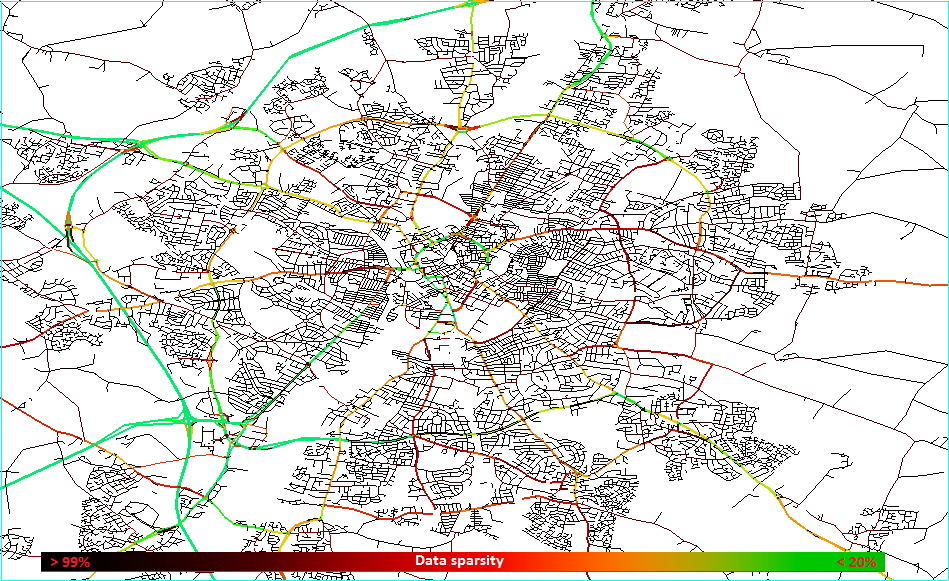
\includegraphics[width=0.7\textwidth]{DataSparsityColorScale}
\caption{Illustrating the data sparsity in the dataset for the traffic network in Leicestershire, UK.}
\label{fig:visualsparsity}
\end{figure*}

\begin{figure}[!t]
\centering
\resizebox{0.48\textwidth}{!}{
\begin{tikzpicture}
		\begin{axis}[
		width=1.0\textwidth,
		height=0.5\textwidth, 
		xlabel={Time of Day}, 
		ylabel={Percentage of Total Links [\%]}, 
		date coordinates in=x, 
		table/col sep=comma, 
		date ZERO=2015-09-13, 
		xticklabel=\hour:\minute, 
		xticklabel style={rotate=50, anchor=near xticklabel},
		legend style={at={(0.5,1)},anchor=north,legend columns=1,legend cell align=left,},
		ymajorgrids=true,
		grid style=dashed,
		ymin=20, 
		ymax=70,
		enlarge x limits=0.1,]
		\addplot[ybar,ybar legend,fill=teal!50] table[x=date,y=value]{sparseratebyhour.csv};\addlegendentry{Time of day vs Number of traffic links having data sparsity $\leq$ 99\%}
		%\addplot[draw=teal,thick,smooth] table[x=date,y=value] {sparseratebyhour.csv};\addlegendentry{Fitting result}
		\end{axis}
		\end{tikzpicture}
}
\caption{Illustration the data sparsity in links by the time of day.}
\label{fig:sparsityplotFCD}
\end{figure}

According to the travel time data that is acquired from Leicestershire from 2009 to 2012, the data sparsity of links visually shows very high values in Figure \ref{fig:visualsparsity} where data sparsity is presented by colour on map for every links. Figure \ref{fig:sparsityplotFCD} indicates that 69.42\% of total links have data sparsity is less than or equal to 99\%. Figure \ref{fig:sparsityplotFCD} shows that the number of travel time samples is different by the time of the day. There are more travel time data for the time interval between 7am and 7pm. NLIM is proposed for large scale traffic networks, hence it should perform well for most of the links in the traffic networks.

The FCD dataset which is a real historical travel time dataset is used to assess the performances of NLIM. The NLIM employed MLR, FF-EL-ANN and FF-RPROP-ANN are trained on the dataset. The performance metrics of NLIM models are given by using unseen data. After that, the performances of NLIM models will be compared to the achievements of NLIM models on three previous datasets. As discussed in the previous section, due to the long training time on a large number of labelled data and less accurate of SVR-LK models, so it is eliminated in this experiment.

To demonstrate the advantages of NLIM models in different machine learning techniques, their performance is compared with those of Historical Average (HA) and Moving Average (MA) methods \cite{Tang2018}. HA and MA are typical standard methods that allow estimating the current travel time by using historical travel time data. HA uses the corresponding average of the historical travel time of a time slot on a target link to estimate the current time slot travel time on the link. Meanwhile, MA uses moving average of three-time slots right before the current time slot to estimate the current time slot travel time \cite{Tang2018}.

Input features for training and testing NLIM models in a link layout using the proposed method are sparse historical travel time of neighbouring links, time of day(time slot), vehicle class and day of a week. Day of a week is inferred from the date. Output feature is travel time corresponding to the input features of a target link.

13527 links produce 13527 link layouts. There are 338177 traffic link models in total. The models  are carefully trained and verified to make sure relationships between temporal and spatial of travel times in links correctly learnt. The performances of models are evaluated by RMSE, MAE and MAPE performance metrics on unseen data. Outliers of data set on 13527 traffic links are detected and removed using the proposed DR-M-GMM (Algorithm \ref{alg:outlieralgorithm}). The parameter $k$ and $\gamma$ are set up as mentioned in Section \ref{NLIMmethod} ($k$ = 5, $\gamma$ = 0.1).
\subsection{Performance criteria}
\subsection{Results}

\begin{figure}[!t]
	\centering
	\captionsetup{justification=centering}
	\begin{tikzpicture}
	\small
	\begin{axis}[
	width=0.9\textwidth,
	height=.7\textwidth,
	grid=both,
	%ymajorgrids=true,
	grid style=dotted,
	x tick label style={/pgf/number format/1000 sep=},
	legend style={at={(0.6,1)},
		anchor=north,legend columns=2},
	axis y line*=left,
	ymin=0,ymax=100,
	xmin=1,xmax=100,
	xlabel={Data sparsity threshold[\%]},
	ylabel style={align=center},
	ylabel={Percentage of links having RMSE of best models $\le$ 3 seconds \\in total links},
	]
	\addplot[color=olive, mdensely dashdotted] table[x=Bin,y=SMS] {NumLinkRMSELE300PerSparseRate.csv}; \label{plot1} \addlegendentry{SMS}
	\addplot[color=orange, mdensely dashed] table[x=Bin,y=FF-EL-ANN] {NumLinkRMSELE300PerSparseRate.csv}; \label{plot2} \addlegendentry{NLIM-EL-OD}
	\addplot[color=blue!80, mloosely dotted] table[x=Bin,y=FF-RPROP-ANN] {NumLinkRMSELE300PerSparseRate.csv}; \label{plot5} \addlegendentry{NLIM-RPROP-OD}
	\addplot[color=cyan, mdashed] table[x=Bin,y=MLR] {NumLinkRMSELE300PerSparseRate.csv}; \label{plot5} \addlegendentry{NLIM-MLR-OD}
	\end{axis}
	\begin{axis}[
	width=0.9\textwidth,
	height=.7\textwidth,
	legend style={at={(0.3,0.12)},legend columns=1},
	axis y line*=right,
	axis x line=none,
	xmin=1,xmax=100,
	ymin=0,ymax=60,
	ylabel={Percentage of Study Links in Traffic Networks[\%]},
	]
	\addplot[color=black!90,mloosely dashdotted] table[x=Bin,y=SparseR] {NumLinkRMSELE300PerSparseRate.csv};\addlegendentry{SRT-Links}
	\end{axis}
	\end{tikzpicture}
	\caption[Percentage of links that have RMSE of the best model less than or equal to 3 seconds vs sparsity threshold]{Percentage of links that have RMSE of the best model less than or equal to 3 seconds vs sparsity threshold achieved by Neighbouring link inference method with similar model searching (SMS), NLIM employed FF-EL-ANN (NLIM-EL-OD), NLIM employed FF-RPROP-ANN (NLIM-RPRO-OD), NLIM employed MLR (NLIM-MLR-OD) on the unseen data. Outliers are identified and removed from the unseen test data by applying Algorithm \ref{alg:outlieralgorithm}.}
	\label{fig:smsperformanceRMSE}
\end{figure} 

\begin{figure*}[!t]
	\centering
	\subfloat[Motorway Links]{
		\begin{tikzpicture}
		\tiny
		\begin{axis}[
		width=0.5\textwidth,
		ymajorgrids=true,
		grid style=dotted,
		major x tick style = transparent,
		legend style={at={(0.5,1)},
			anchor=north,legend columns=1},
		ymin=0,ymax=35,
		xmin=0.6,xmax=4.9,
		ylabel = {MAPE [\%]},
		xticklabels={(1), (2), (3), (4)},
		xtick={1.3,2.3,3.3,4.3, 5.3},
		boxplot/draw direction=y,
		scatter/classes={%
			a={mark=o,draw=cyan},
			b={mark=diamond,draw=orange},
			c={mark=star,draw=blue!80},
			d={mark=triangle,olive}
		},
		]
		
		\addplot[color=cyan, dash pattern=on 4pt off 3pt,] table[y=Bin,x=motorwayMLR] {all-hist-MAPE.csv};
		\addplot[color=orange, dash pattern=on 2pt off 2pt,] table[y=Bin,x=motorwayEL] {all-hist-MAPE.csv};
		\addplot[color=blue!80, dash pattern=on 4pt off 1pt,] table[y=Bin,x=motorwayRPROP] {all-hist-MAPE.csv};
		\addplot[color=olive, dash pattern=on 2pt off 1pt,line width=0.45mm,] table[y=Bin,x=motorwaySMS] {all-hist-MAPE.csv};
		
		\addplot[scatter,only marks, scatter src=explicit symbolic, mark size=2,] table[meta=label] {MAPEmotorwayMLR.csv};
		\addplot[scatter,only marks, scatter src=explicit symbolic, mark size=2,] table[meta=label] {MAPEmotorwayEL.csv};
		\addplot[scatter,only marks, scatter src=explicit symbolic, mark size=2,] table[meta=label] {MAPEmotorwayRPROP.csv};
		\addplot[scatter,only marks, scatter src=explicit symbolic, mark size=2,] table[meta=label] {MAPEmotorwaySMS.csv};
		
		\addplot+[boxplot prepared={
			lower whisker=8.07817702351881, lower quartile= 9.36723648776469, median= 10.3549469462742, upper quartile= 12.5550845177071, upper whisker= 56.8557687430948,
			box extend=0.2,every box/.style={fill=cyan!20}}, color=cyan, dash pattern=on 4pt off 3pt,]
		coordinates {};
		\addplot+[boxplot prepared={
			lower whisker=3.72863573835834, lower quartile= 8.03574347088319, median= 9.32633854865565, upper quartile= 11.4637040680264, upper whisker= 50.5138750065698,
			box extend=0.2,every box/.style={fill=orange!20}}, color=orange, dash pattern=on 2pt off 2pt,]
		coordinates {};
		\addplot+[boxplot prepared={
			lower whisker=1.27496162405221, lower quartile= 3.56984170937629, median= 8.08220917099729, upper quartile= 10.8464894380275, upper whisker= 50.2227588815785,
			box extend=0.2,every box/.style={fill=blue!20}}, color=blue!80, dash pattern=on 4pt off 1pt,]
		coordinates {};
		\addplot+[boxplot prepared={
			lower whisker=1.27496162405221, lower quartile= 2.55923298066818, median= 4.21127069889067, upper quartile= 7.06435588816994, upper whisker= 51.7793019196893,
			box extend=0.2,every box/.style={fill=olive!20}}, color=olive, dash pattern=on 1pt off 1pt,]
		coordinates {};
		\end{axis}
		\end{tikzpicture}
	}
	\subfloat[Trunk Links]{
		\begin{tikzpicture}
		\tiny
		\begin{axis}[
		width=0.5\textwidth,
		ymajorgrids=true,
		grid style=dotted,
		major x tick style = transparent,
		legend style={at={(0.5,1)},
			anchor=north,legend columns=1},
		ymin=0,ymax=35,
		xmin=0.6,xmax=4.9,
		ylabel = {MAPE [\%]},
		xticklabels={(1), (2), (3), (4)},
		xtick={1.3,2.3,3.3,4.3},
		boxplot/draw direction=y,
		scatter/classes={%
			a={mark=o,draw=cyan},
			b={mark=diamond,draw=orange},
			c={mark=star,draw=blue!80},
			d={mark=triangle,olive}
		},
		]
		
		\addplot[color=cyan, dash pattern=on 4pt off 3pt,] table[y=Bin,x=trunkMLR] {all-hist-MAPE.csv};
		\addplot[color=orange, dash pattern=on 2pt off 2pt,] table[y=Bin,x=trunkEL] {all-hist-MAPE.csv};
		\addplot[color=blue!80, dash pattern=on 4pt off 1pt,] table[y=Bin,x=trunkRPROP] {all-hist-MAPE.csv};
		\addplot[color=olive, dash pattern=on 2pt off 1pt,line width=0.45mm,] table[y=Bin,x=trunkSMS] {all-hist-MAPE.csv};
		
		\addplot[scatter,only marks, scatter src=explicit symbolic, mark size=2,] table[meta=label] {MAPEtrunkMLR.csv};
		\addplot[scatter,only marks, scatter src=explicit symbolic, mark size=2,] table[meta=label] {MAPEtrunkEL.csv};
		\addplot[scatter,only marks, scatter src=explicit symbolic, mark size=2,] table[meta=label] {MAPEtrunkRPROP.csv};
		\addplot[scatter,only marks, scatter src=explicit symbolic, mark size=2,] table[meta=label] {MAPEtrunkSMS.csv};
		
		\addplot+[boxplot prepared={
			lower whisker=12.6526552613753, lower quartile= 13.2196850971613, median= 14.3704935770663, upper quartile= 17.2841270272597, upper whisker= 30.9022373015265,
			box extend=0.2,every box/.style={fill=cyan!20}}, color=cyan, dash pattern=on 4pt off 3pt,]
		coordinates {};
		\addplot+[boxplot prepared={
			lower whisker=8.13569251270077, lower quartile= 9.13341258947368, median= 10.2615958947885, upper quartile= 13.4387362118007, upper whisker= 24.8665028856083,
			box extend=0.2,every box/.style={fill=orange!20}}, color=orange, dash pattern=on 2pt off 2pt,]
		coordinates {};
		\addplot+[boxplot prepared={
			lower whisker=5.42666155639375, lower quartile= 8.65331145134375, median= 9.70769548106881, upper quartile= 12.8049953228403, upper whisker= 21.7697226461666,
			box extend=0.2,every box/.style={fill=blue!20}}, color=blue!80, dash pattern=on 4pt off 1pt,]
		coordinates {};
		\addplot+[boxplot prepared={
			lower whisker=5.42666155639375, lower quartile= 6.15202970952085, median= 7.49723641714504, upper quartile= 11.3315837259506, upper whisker= 21.7697226461666,
			box extend=0.2,every box/.style={fill=olive!20}}, color=olive, dash pattern=on 2pt off 1pt,]
		coordinates {};
		\end{axis}
		\end{tikzpicture}
	}
	\hfill
	\subfloat[Primary Links]{
		\begin{tikzpicture}
		\tiny
		\begin{axis}[
		width=0.5\textwidth,
		ymajorgrids=true,
		grid style=dotted,
		major x tick style = transparent,
		legend style={at={(0.5,1)},
			anchor=north,legend columns=1},
		ymin=0,ymax=35,
		xmin=0.6,xmax=4.9,
		ylabel = {MAPE [\%]},
		xticklabels={(1),(2),(3),(4)},
		xtick={1.3,2.3,3.3,4.3},
		boxplot/draw direction=y,
		scatter/classes={%
			a={mark=o,draw=cyan},
			b={mark=diamond,draw=orange},
			c={mark=star,draw=blue!80},
			d={mark=triangle,olive}
		},
		]
		
		\addplot[color=cyan, dash pattern=on 4pt off 3pt,] table[y=Bin,x=primaryMLR] {all-hist-MAPE.csv};
		\addplot[color=orange, dash pattern=on 2pt off 2pt,] table[y=Bin,x=primaryEL] {all-hist-MAPE.csv};
		\addplot[color=blue!80, dash pattern=on 4pt off 1pt,] table[y=Bin,x=primaryRPROP] {all-hist-MAPE.csv};
		\addplot[color=olive, dash pattern=on 2pt off 1pt,line width=0.45mm,] table[y=Bin,x=primarySMS] {all-hist-MAPE.csv};
		
		\addplot[scatter,only marks, scatter src=explicit symbolic, mark size=2,] table[meta=label] {MAPEprimaryMLR.csv};
		\addplot[scatter,only marks, scatter src=explicit symbolic, mark size=2,] table[meta=label] {MAPEprimaryEL.csv};
		\addplot[scatter,only marks, scatter src=explicit symbolic, mark size=2,] table[meta=label] {MAPEprimaryRPROP.csv};
		\addplot[scatter,only marks, scatter src=explicit symbolic, mark size=2,] table[meta=label] {MAPEprimarySMS.csv};
		
		\addplot+[boxplot prepared={
			lower whisker=10.83567235529, lower quartile= 12.6976062339961, median= 16.625413435691, upper quartile= 19.3514417135242, upper whisker= 37.554679136981,
			box extend=0.2,every box/.style={fill=cyan!20}}, color=cyan, dash pattern=on 4pt off 3pt,]
		coordinates {};
		\addplot+[boxplot prepared={
			lower whisker=6.83715964262968, lower quartile= 9.68192999070953, median= 12.6345447676676, upper quartile= 14.8772977665848, upper whisker= 21.9153864537951,
			box extend=0.2,every box/.style={fill=orange!20}}, color=orange, dash pattern=on 2pt off 2pt,]
		coordinates {};
		\addplot+[boxplot prepared={
			lower whisker=5.17432446003648, lower quartile= 8.73274991173785, median= 11.2848047042072, upper quartile= 14.4828182464181, upper whisker= 25.5334921112125,
			box extend=0.2,every box/.style={fill=blue!20}}, color=blue!80, dash pattern=on 4pt off 1pt,]
		coordinates {};
		\addplot+[boxplot prepared={
			lower whisker=3.62201452051871, lower quartile= 5.83345287530273, median= 10.4856030489892, upper quartile= 13.54989719144, upper whisker= 20.3968507871448,
			box extend=0.2,every box/.style={fill=olive!20}}, color=olive, dash pattern=on 2pt off 1pt,]
		coordinates {};
		\end{axis}
		\end{tikzpicture}
	}
	\subfloat[A Links]{
		\begin{tikzpicture}
		\tiny
		\begin{axis}[
		width=0.5\textwidth,
		ymajorgrids=true,
		grid style=dotted,
		major x tick style = transparent,
		legend style={at={(0.5,1)},
			anchor=north,legend columns=1},
		ymin=0,ymax=35,
		xmin=0.6,xmax=4.9,
		ylabel = {MAPE [\%]},
		xticklabels={(1),(2),(3),(4)},
		xtick={1.3,2.3,3.3,4.3},
		boxplot/draw direction=y,
		scatter/classes={%
			a={mark=o,draw=cyan},
			b={mark=diamond,draw=orange},
			c={mark=star,draw=blue!80},
			d={mark=triangle,olive}
		},
		]
		
		\addplot[color=cyan, dash pattern=on 4pt off 3pt,] table[y=Bin,x=aMLR] {all-hist-MAPE.csv};
		\addplot[color=orange, dash pattern=on 2pt off 2pt,] table[y=Bin,x=aEL] {all-hist-MAPE.csv};
		\addplot[color=blue!80, dash pattern=on 4pt off 1pt,] table[y=Bin,x=aRPROP] {all-hist-MAPE.csv};
		\addplot[color=olive, dash pattern=on 2pt off 1pt,line width=0.45mm,] table[y=Bin,x=aSMS] {all-hist-MAPE.csv};
		
		\addplot[scatter,only marks, scatter src=explicit symbolic, mark size=2,] table[meta=label] {MAPEaMLR.csv};
		\addplot[scatter,only marks, scatter src=explicit symbolic, mark size=2,] table[meta=label] {MAPEaEL.csv};
		\addplot[scatter,only marks, scatter src=explicit symbolic, mark size=2,] table[meta=label] {MAPEaRPROP.csv};
		\addplot[scatter,only marks, scatter src=explicit symbolic, mark size=2,] table[meta=label] {MAPEaSMS.csv};
		
		\addplot+[boxplot prepared={
			lower whisker=10.6850241937262, lower quartile= 13.9819864718904, median= 18.102006023278, upper quartile= 28.0721067617297, upper whisker= 233.413610870536,
			box extend=0.2,every box/.style={fill=cyan!20}}, color=cyan, dash pattern=on 4pt off 3pt,]
		coordinates {};
		\addplot+[boxplot prepared={
			lower whisker=6.69525937751067, lower quartile= 12.5544903623061, median= 16.8783985008471, upper quartile= 23.0863318565223, upper whisker= 237.883696059368,
			box extend=0.2,every box/.style={fill=orange!20}}, color=orange, dash pattern=on 2pt off 2pt,]
		coordinates {};
		\addplot+[boxplot prepared={
			lower whisker=3.77441234853988, lower quartile= 11.5045541900333, median= 15.7015423752324, upper quartile= 24.2207108934723, upper whisker= 164.759787561683,
			box extend=0.2,every box/.style={fill=blue!20}}, color=blue!80, dash pattern=on 4pt off 1pt,]
		coordinates {};
		\addplot+[boxplot prepared={
			lower whisker=2.37553098921991, lower quartile= 6.38287742591445, median= 10.1327574765387, upper quartile= 19.2933322609827, upper whisker= 112.596193951848,
			box extend=0.2,every box/.style={fill=olive!20}}, color=olive, dash pattern=on 2pt off 1pt,]
		coordinates {};
		\end{axis}
		\end{tikzpicture}
	}
	\hfill
	\subfloat[B Links]{
		\begin{tikzpicture}
		\tiny
		\begin{axis}[
		width=0.5\textwidth,
		ymajorgrids=true,
		grid style=dotted,
		major x tick style = transparent,
		legend style={at={(0.5,1)},
			anchor=north,legend columns=1},
		ymin=0,ymax=35,
		xmin=0.6,xmax=4.9,
		ylabel = {MAPE [\%]},
		xticklabels={(1),(2),(3),(4)},
		xtick={1.3,2.3,3.3,4.3},
		boxplot/draw direction=y,
		scatter/classes={%
			a={mark=o,draw=cyan},
			b={mark=diamond,draw=orange},
			c={mark=star,draw=blue!80},
			d={mark=triangle,olive}
		},
		]
		
		\addplot[color=cyan, dash pattern=on 4pt off 3pt,] table[y=Bin,x=bMLR] {all-hist-MAPE.csv};
		\addplot[color=orange, dash pattern=on 2pt off 2pt,] table[y=Bin,x=bEL] {all-hist-MAPE.csv};
		\addplot[color=blue!80, dash pattern=on 4pt off 1pt,] table[y=Bin,x=bRPROP] {all-hist-MAPE.csv};
		\addplot[color=olive, dash pattern=on 2pt off 1pt,line width=0.45mm,] table[y=Bin,x=bSMS] {all-hist-MAPE.csv};
		
		\addplot[scatter,only marks, scatter src=explicit symbolic, mark size=2,] table[meta=label] {MAPEbMLR.csv};
		\addplot[scatter,only marks, scatter src=explicit symbolic, mark size=2,] table[meta=label] {MAPEbEL.csv};
		\addplot[scatter,only marks, scatter src=explicit symbolic, mark size=2,] table[meta=label] {MAPEbRPROP.csv};
		\addplot[scatter,only marks, scatter src=explicit symbolic, mark size=2,] table[meta=label] {MAPEbSMS.csv};
		
		\addplot+[boxplot prepared={
			lower whisker=11.2150059168673, lower quartile= 16.579636853878, median= 19.1246780902686, upper quartile= 24.1442191037081, upper whisker= 298.289707863304,
			box extend=0.2,every box/.style={fill=cyan!20}}, color=cyan, dash pattern=on 4pt off 3pt,]
		coordinates {};
		\addplot+[boxplot prepared={
			lower whisker=6.41295567960272, lower quartile= 11.6693291367129, median= 14.8866942367983, upper quartile= 21.2030898958226, upper whisker= 317.670628396456,
			box extend=0.2,every box/.style={fill=orange!20}}, color=orange, dash pattern=on 2pt off 2pt,]
		coordinates {};
		\addplot+[boxplot prepared={
			lower whisker=5.87618907240655, lower quartile= 11.4183184358475, median= 14.5230502137893, upper quartile= 20.8279634433645, upper whisker= 149.324152591167,
			box extend=0.2,every box/.style={fill=blue!20}}, color=blue!80, dash pattern=on 4pt off 1pt,]
		coordinates {};
		\addplot+[boxplot prepared={
			lower whisker=3.29189547855424, lower quartile= 9.0006382194903, median= 11.2700280296142, upper quartile= 15.7893354471255, upper whisker= 220.507074230819,
			box extend=0.2,every box/.style={fill=olive!20}}, color=olive, dash pattern=on 2pt off 1pt,]
		coordinates {};
		\end{axis}
		\end{tikzpicture}
	}
	\subfloat[Minor Links]{
		\begin{tikzpicture}
		\tiny
		\begin{axis}[
		width=0.5\textwidth,
		ymajorgrids=true,
		grid style=dotted,
		major x tick style = transparent,
		legend style={at={(0.5,1)},
			anchor=north,legend columns=1},
		ymin=0,ymax=35,
		xmin=0.6,xmax=4.9,
		ylabel = {MAPE [\%]},
		xticklabels={(1),(2),(3),(4)},
		xtick={1.3,2.3,3.3,4.3},
		boxplot/draw direction=y,
		scatter/classes={%
			a={mark=o,draw=cyan},
			b={mark=diamond,draw=orange},
			c={mark=star,draw=blue!80},
			d={mark=triangle,olive}
		},
		]
		
		\addplot[color=cyan, dash pattern=on 4pt off 3pt,] table[y=Bin,x=minorMLR] {all-hist-MAPE.csv};
		\addplot[color=orange, dash pattern=on 2pt off 2pt,] table[y=Bin,x=minorEL] {all-hist-MAPE.csv};
		\addplot[color=blue!80, dash pattern=on 4pt off 1pt,] table[y=Bin,x=minorRPROP] {all-hist-MAPE.csv};
		\addplot[color=olive, dash pattern=on 2pt off 1pt,line width=0.45mm,] table[y=Bin,x=minorSMS] {all-hist-MAPE.csv};
		
		\addplot[scatter,only marks, scatter src=explicit symbolic, mark size=2,] table[meta=label] {MAPEminorMLR.csv};
		\addplot[scatter,only marks, scatter src=explicit symbolic, mark size=2,] table[meta=label] {MAPEminorEL.csv};
		\addplot[scatter,only marks, scatter src=explicit symbolic, mark size=2,] table[meta=label] {MAPEminorRPROP.csv};
		\addplot[scatter,only marks, scatter src=explicit symbolic, mark size=2,] table[meta=label] {MAPEminorSMS.csv};
		
		\addplot+[boxplot prepared={
			lower whisker=9.29360870142, lower quartile= 14.7123892707262, median= 17.9835963528661, upper quartile= 22.6623852637501, upper whisker= 200.989701267327,
			box extend=0.2,every box/.style={fill=cyan!20}}, color=cyan, dash pattern=on 4pt off 3pt,]
		coordinates {};
		\addplot+[boxplot prepared={
			lower whisker=3.07398992127296, lower quartile= 10.4954501440983, median= 12.9306213286707, upper quartile= 17.2358403358054, upper whisker= 153.287113153354,
			box extend=0.2,every box/.style={fill=orange!20}}, color=orange, dash pattern=on 2pt off 2pt,]
		coordinates {};
		\addplot+[boxplot prepared={
			lower whisker=2.50380995607164, lower quartile= 10.000476682215, median= 12.8774757322803, upper quartile= 17.3148419665041, upper whisker= 442.246325847833,
			box extend=0.2,every box/.style={fill=blue!20}}, color=blue!80, dash pattern=on 4pt off 1pt,]
		coordinates {};
		\addplot+[boxplot prepared={
			lower whisker=0.803957162155631, lower quartile= 6.1005338671709, median= 8.88576023034912, upper quartile= 13.3600667960694, upper whisker= 149.837082511949,
			box extend=0.2,every box/.style={fill=olive!20}}, color=olive, dash pattern=on 2pt off 1pt,]
		coordinates {};
		\end{axis}
		\end{tikzpicture}
	}
	\hfill
	\caption[Density of the best NLIM models of individual link type and their MAPEs (\%) achieved on experiment 4 unseen data]{Density of the best NLIM models, different machine learning techniques applied, of Motorway (a), Trunk (b), Primary (c), A (d), B (e) and Minor (f) links and their MAPEs [\%] achieved on unseen data. Sub-figures are in the same scale. (1) is for MLR, (2) is for FF-EL-ANN, (3) is for FF-RPROP-ANN and (4) is for SMS. The density of best models in each method is presented by boxplot (lower whisker, lower quartile, median, upper quartile, upper whisker), visualisation of the actual individual model and the histogram of the models respectively. Some high MAPE data points are out of the figure, hence corresponding upper-whiskers can not be shown.}
	\label{fig:smspeformancespsecificlinkcateogry}
\end{figure*}

% An example of a floating figure using the graphicx package.
% Note that \label must occur AFTER (or within) \caption.
% For figures, \caption should occur after the \includegraphics.
% Note that IEEEtran v1.7 and later has special internal code that
% is designed to preserve the operation of \label within \caption
% even when the captionsoff option is in effect. However, because
% of issues like this, it may be the safest practice to put all your
% \label just after \caption rather than within \caption{}.
%
% Reminder: the "draftcls" or "draftclsnofoot", not "draft", class
% option should be used if it is desired that the figures are to be
% displayed while in draft mode.
%
%\begin{figure}[!t]
%\centering
%\includegraphics[width=2.5in]{myfigure}
% where an .eps filename suffix will be assumed under latex, 
% and a .pdf suffix will be assumed for pdflatex; or what has been declared
% via \DeclareGraphicsExtensions.
%\caption{Simulation results for the network.}
%\label{fig_sim}
%\end{figure}

% Note that the IEEE typically puts floats only at the top, even when this
% results in a large percentage of a column being occupied by floats.


% An example of a double column floating figure using two subfigures.
% (The subfig.sty package must be loaded for this to work.)
% The subfigure \label commands are set within each subfloat command,
% and the \label for the overall figure must come after \caption.
% \hfil is used as a separator to get equal spacing.
% Watch out that the combined width of all the subfigures on a 
% line do not exceed the text width or a line break will occur.
%
%\begin{figure*}[!t]
%\centering
%\subfloat[Case I]{\includegraphics[width=2.5in]{box}%
%\label{fig_first_case}}
%\hfil
%\subfloat[Case II]{\includegraphics[width=2.5in]{box}%
%\label{fig_second_case}}
%\caption{Simulation results for the network.}
%\label{fig_sim}
%\end{figure*}
%
% Note that often IEEE papers with subfigures do not employ subfigure
% captions (using the optional argument to \subfloat[]), but instead will
% reference/describe all of them (a), (b), etc., within the main caption.
% Be aware that for subfig.sty to generate the (a), (b), etc., subfigure
% labels, the optional argument to \subfloat must be present. If a
% subcaption is not desired, just leave its contents blank,
% e.g., \subfloat[].


% An example of a floating table. Note that, for IEEE style tables, the
% \caption command should come BEFORE the table and, given that table
% captions serve much like titles, are usually capitalized except for words
% such as a, an, and, as, at, but, by, for, in, nor, of, on, or, the, to
% and up, which are usually not capitalized unless they are the first or
% last word of the caption. Table text will default to \footnotesize as
% the IEEE normally uses this smaller font for tables.
% The \label must come after \caption as always.
%
%\begin{table}[!t]
%% increase table row spacing, adjust to taste
%%\renewcommand{\arraystretch}{1.3}
%% if using array.sty, it might be a good idea to tweak the value of
%% \extrarowheight as needed to properly center the text within the cells
%\caption{An Example of a Table}
%\label{table_example}
%\centering
%% Some packages, such as MDW tools, offer better commands for making tables
%% than the plain LaTeX2e tabular which is used here.
%\begin{tabular}{|c||c|}
%\hline
%One & Two\\
%\hline
%Three & Four\\
%\hline
%\end{tabular}
%\end{table}


% Note that the IEEE does not put floats in the very first column
% - or typically anywhere on the first page for that matter. Also,
% in-text middle ("here") positioning is typically not used, but it
% is allowed and encouraged for Computer Society conferences (but
% not Computer Society journals). Most IEEE journals/conferences use
% top floats exclusively. 
% Note that, LaTeX2e, unlike IEEE journals/conferences, places
% footnotes above bottom floats. This can be corrected via the
% \fnbelowfloat command of the stfloats package.




\section{Conclusions} 
\label{sec:conclusions}
Improving the performance of NLIM in minor links which have datasets with high data sparsity and irregularity links has been considered in this section. The main idea is to adapt travel time data of similar NLIM models to improve a selected NLIM model.
The similar model searching (SMS) has been evaluated on FCD dataset. NLIM was firstly used for traffic links to create a collection of NLIM models. Then, the similar model searching method was applied. Results show that SMS is capable of improving
the performance of NLIM on learning the temporal and spatial relationship between the travel time of a target link and travel time of its neighbouring link despite the high data sparsity and irregularity of the dataset.



% if have a single appendix:
\appendix[Algorithms]
% or
%\appendix  % for no appendix heading
% do not use \section anymore after \appendix, only \section*
% is possibly needed

% use appendices with more than one appendix
% then use \section to start each appendix
% you must declare a \section before using any
% \subsection or using \label (\appendices by itself
% starts a section numbered zero.)
%


%\appendices
%\section{Algorithms}


% you can choose not to have a title for an appendix
% if you want by leaving the argument blank
%\section{}
%Appendix two text goes here.


% use section* for acknowledgment
\section*{Acknowledgment}
This work was supported by the Polish National Science Centre under grant no. DEC-2016/21/B/HS4/00667


% Can use something like this to put references on a page
% by themselves when using endfloat and the captionsoff option.
\ifCLASSOPTIONcaptionsoff
  \newpage
\fi



% trigger a \newpage just before the given reference
% number - used to balance the columns on the last page
% adjust value as needed - may need to be readjusted if
% the document is modified later
%\IEEEtriggeratref{8}
% The "triggered" command can be changed if desired:
%\IEEEtriggercmd{\enlargethispage{-5in}}

% references section

% can use a bibliography generated by BibTeX as a .bbl file
% BibTeX documentation can be easily obtained at:
% http://mirror.ctan.org/biblio/bibtex/contrib/doc/
% The IEEEtran BibTeX style support page is at:
% http://www.michaelshell.org/tex/ieeetran/bibtex/
%\bibliographystyle{IEEEtran}
% argument is your BibTeX string definitions and bibliography database(s)
%\bibliography{IEEEabrv,../bib/paper}
%
% <OR> manually copy in the resultant .bbl file
% set second argument of \begin to the number of references
% (used to reserve space for the reference number labels box)
%\begin{thebibliography}{1}
%
%\bibitem{IEEEhowto:kopka}
%H.~Kopka and P.~W. Daly, \emph{A Guide to \LaTeX}, 3rd~ed.\hskip 1em plus
%  0.5em minus 0.4em\relax Harlow, England: Addison-Wesley, 1999.
%
%\end{thebibliography}
\bibliographystyle{IEEEtran}

\bibliography{IEEEabrv,../LiteratureReview}
% biography section
% 
% If you have an EPS/PDF photo (graphicx package needed) extra braces are
% needed around the contents of the optional argument to biography to prevent
% the LaTeX parser from getting confused when it sees the complicated
% \includegraphics command within an optional argument. (You could create
% your own custom macro containing the \includegraphics command to make things
% simpler here.)
%\begin{IEEEbiography}[{\includegraphics[width=1in,height=1.25in,clip,keepaspectratio]{mshell}}]{Michael Shell}
% or if you just want to reserve a space for a photo:

\begin{IEEEbiography}{Luong H. Vu}
received the B.S. in Information Technology from University of Information and Communication Technology, Thai Nguyen, Viet Nam, in 2007, and the M.Sc. in Information Technology from Batangas State University, Philippines in 2011. He is currently pursuing the Ph.D. degree with DIGITS, De Montfort University, Leicester, UK. His current interest include intelligent transport systems and computational intelligence.
\end{IEEEbiography}

% if you will not have a photo at all:
\begin{IEEEbiographynophoto}{Benjamin N. Passow}
is a Research and Development Engineer, ITK Engineering, Germany, and a part-time lecturer in Computational Intelligence and Robotics at De Montfort University in Leicester, UK. He received the M.Sc. degree in 2007 and the Ph.D. degree in 2011, both in Computational Intelligence and Robotics from De Montfort University. He is research active within the fields of AI/CI, Transport and Robotics and has participated in various UK, EU and ESA funded projects. In 2009 he received the Machine Intelligence Award from the British Computer Society in Cambridge. His research interests include the theory and application of computational intelligence in intelligent transport, acoustic sensing, autonomous mobile robots, unmanned aerial vehicles, and embedded systems.
\end{IEEEbiographynophoto}

\begin{IEEEbiographynophoto}{Daniel Paluszczyszyn}
received the B.Eng. in Computer Engineering from the University of Zielona Gora, Poland, in 2003, and the M.Sc. in Systems and Control from the Coventry University, UK, in 2008.
From April 2008 till October 2009 he was a Research Assistant at Coventry University developing and implementing a control strategy for a radiotherapy treatment machine. In 2015 he was awarded with the Ph.D. in Hydroinformatics from De Montfort University where he worked as a Research Fellow from 2011 to 2015 in a number of research and commercial projects. Currently, he is working at De Montfort University as a Senior Lecturer in the School of Engineering and Sustainable Development. His recent research interests consider various aspects of intelligent mobility including optimisation of the energy management system for low carbon vehicles and scheduling approaches to charge autonomous electric vehicles.
\end{IEEEbiographynophoto}

\begin{IEEEbiographynophoto}{Lipika Deka}
is a Computer Engineer, currently conducting research within the field of Intelligent Transport Systems and Connected Autonomous Cars. With an educational background in Computer Science and Engineering, PhD in the field of Concurrency Control within File Systems, she has interdisciplinary research experience of applying Computer Science algorithms (mainly AI techniques) in the fields of Chemical Engineering, Healthcare Infrastructure and Intelligent Transport Systems. Presently, she is working on the Software Engineering, Software update, positioning accuracy and path planning aspects of Connected Autonomous Cars.
\end{IEEEbiographynophoto}

\begin{IEEEbiographynophoto}{Eric Goodyer}
is a Professor of Instrumentation. His specialist area of expertise is the design and development of real time instrumentation for industrial, automotive and laboratory use. This is best summed up as ’Measurement Automation and Control’. His research interests are the development of new electromechanical and electronic measuring equipment, and telematic solutions for industry. He works part time for De Montfort University. He also works as a self employed freelance design engineer in my specialist fields, offering design and consultancy service to industry world-wide.
\end{IEEEbiographynophoto}
% insert where needed to balance the two columns on the last page with
% biographies
%\newpage

% You can push biographies down or up by placing
% a \vfill before or after them. The appropriate
% use of \vfill depends on what kind of text is
% on the last page and whether or not the columns
% are being equalized.

%\vfill

% Can be used to pull up biographies so that the bottom of the last one
% is flush with the other column.
%\enlargethispage{-5in}

% that's all folks
\end{document}


